\chapter{Analysis}
The purpose of this chapter is to compare the SRS data structure to the kd-tree. We are going to perform a variety of tests on the SRS data structure and the kd-tree in order to determine the run-time properties of both, mainly looking at when the SRS data structure performs better than the kd-tree.


In order to compare these two data structure random data will be generated and given as input to both, such that both operate on the exact same data. When running a specific test, different data sets are generated during such that one tests is not only performed one a single data set. When the size of a slice has been determined, the search will be performed different places in the data structure such that not only best-case or worst-case scenarios occur. Finally the average of all the searches are returned as the result of the test.


\section{Vertical and horizontal slices}
The first thing to be tested is how big the vertical and horizontal slices can become before the SRS data structure performs worse than the kd-tree. We are going to look at the horizontal slices first.


\begin{figure}[h]
    \centering
    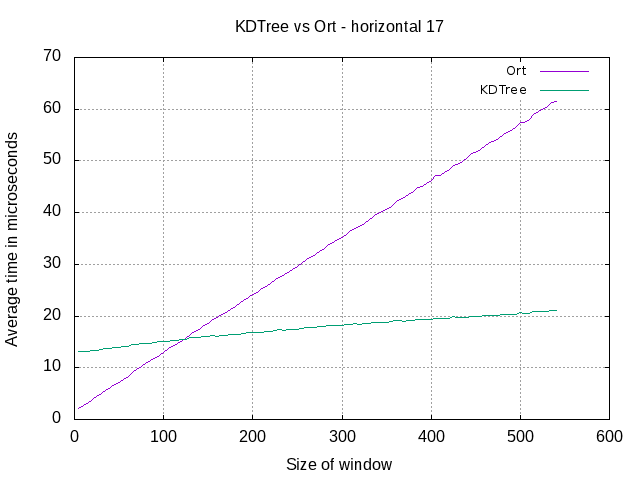
\includegraphics[width = 0.85\textwidth]{pictures/analysis/hori_17.png}
    \caption{Horizontal slice on SRS and kd-tree - data set size of $n=2^{17}$}\label{fig:hori_17}
\end{figure}


\begin{figure}[h]
    \centering
    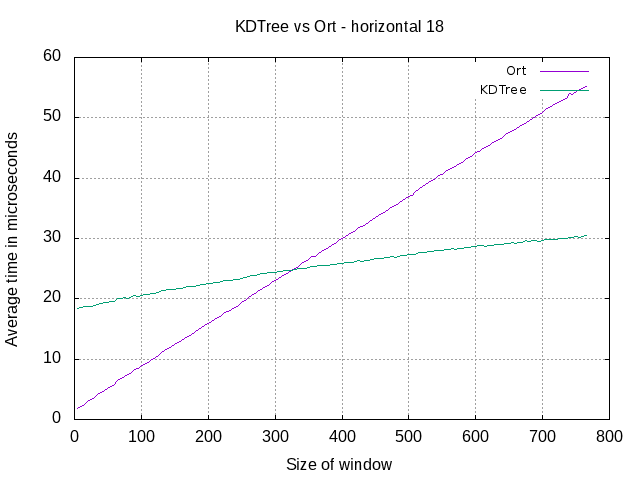
\includegraphics[width = 0.85\textwidth]{pictures/analysis/hori_18.png}
    \caption{Horizontal slice on SRS and kd-tree - data set size of $n=2^{18}$}\label{fig:hori_18}
\end{figure}


\begin{figure}[h]
    \centering
    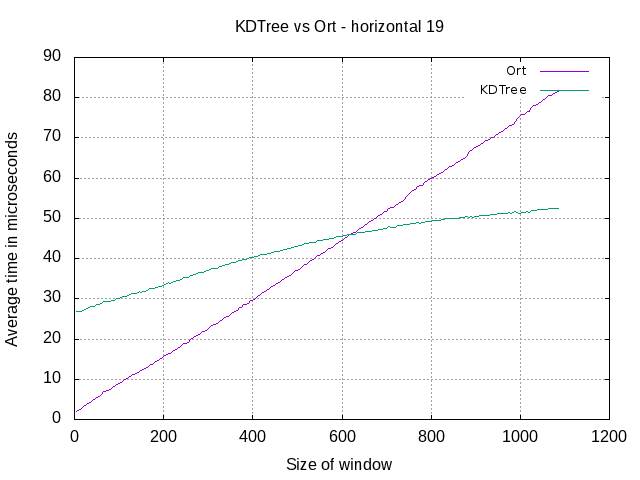
\includegraphics[width = 0.85\textwidth]{pictures/analysis/hori_19.png}
    \caption{Horizontal slice on SRS and kd-tree - data set size of $n=2^{19}$}\label{fig:hori_19}
\end{figure}


\begin{figure}[h]
    \centering
    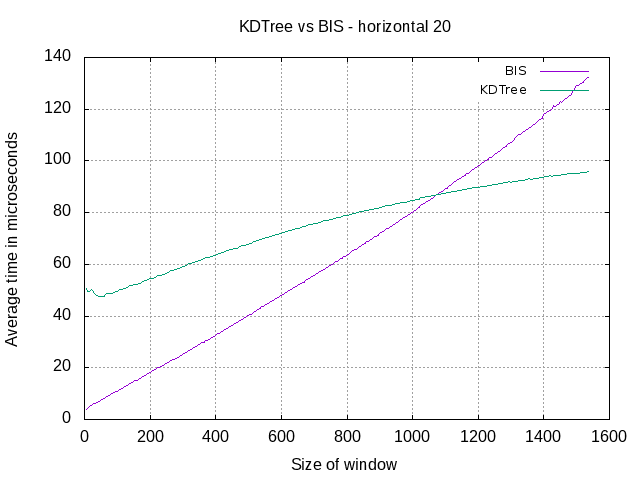
\includegraphics[width = 0.85\textwidth]{pictures/analysis/hori_20.png}
    \caption{Horizontal slice on SRS and kd-tree - data set size of $n=2^{20}$}\label{fig:hori_20}
\end{figure}


\begin{figure}[h]
    \centering
    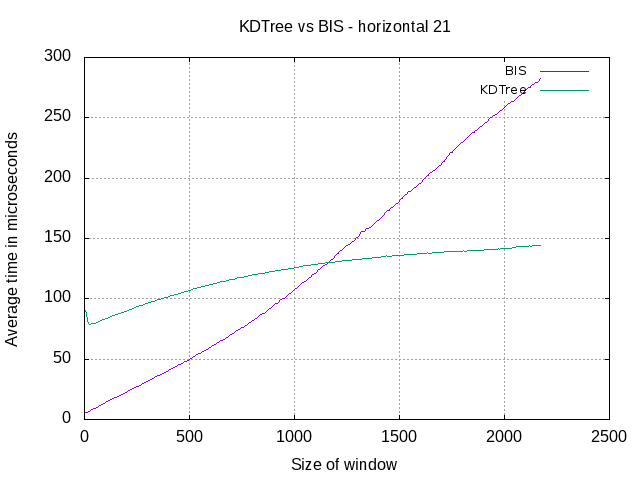
\includegraphics[width = 0.85\textwidth]{pictures/analysis/hori_21.png}
    \caption{Horizontal slice on SRS and kd-tree - data set size of $n=2^{21}$}\label{fig:hori_21}
\end{figure}
\begin{figure}[h]
    \centering
    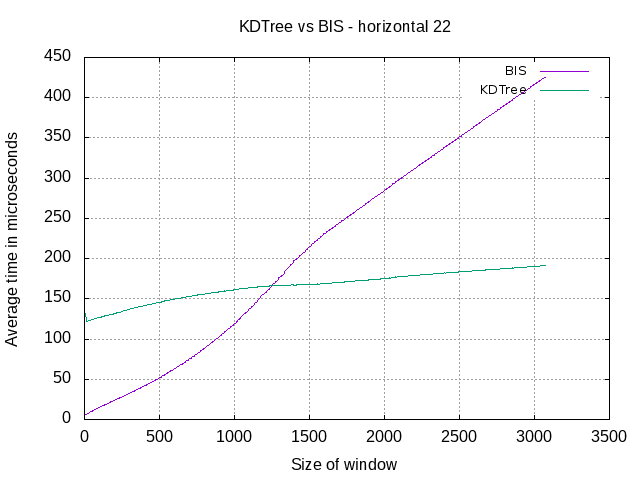
\includegraphics[width = 0.85\textwidth]{pictures/analysis/hori_22.png}
    \caption{Horizontal slice on SRS and kd-tree - data set size of $n=2^{22}$}\label{fig:hori_22}
\end{figure}
\begin{figure}[h]
    \centering
    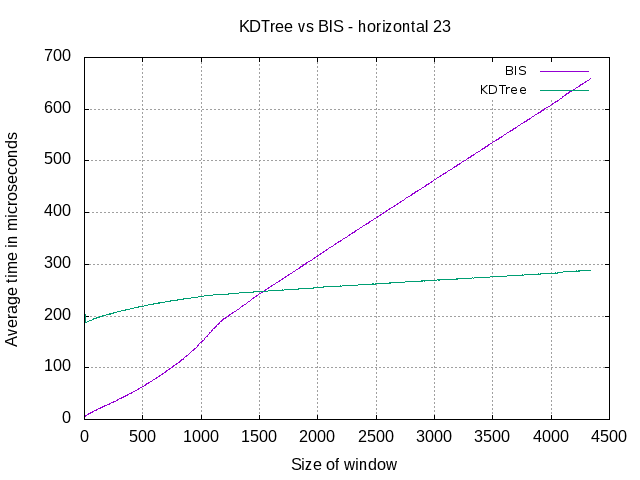
\includegraphics[width = 0.85\textwidth]{pictures/analysis/hori_23.png}
    \caption{Horizontal slice on SRS and kd-tree - data set size of $n=2^{23}$}\label{fig:hori_23}
\end{figure}
